% !TEX root = ./main.tex
\begin{figure}[h]
    \centering
    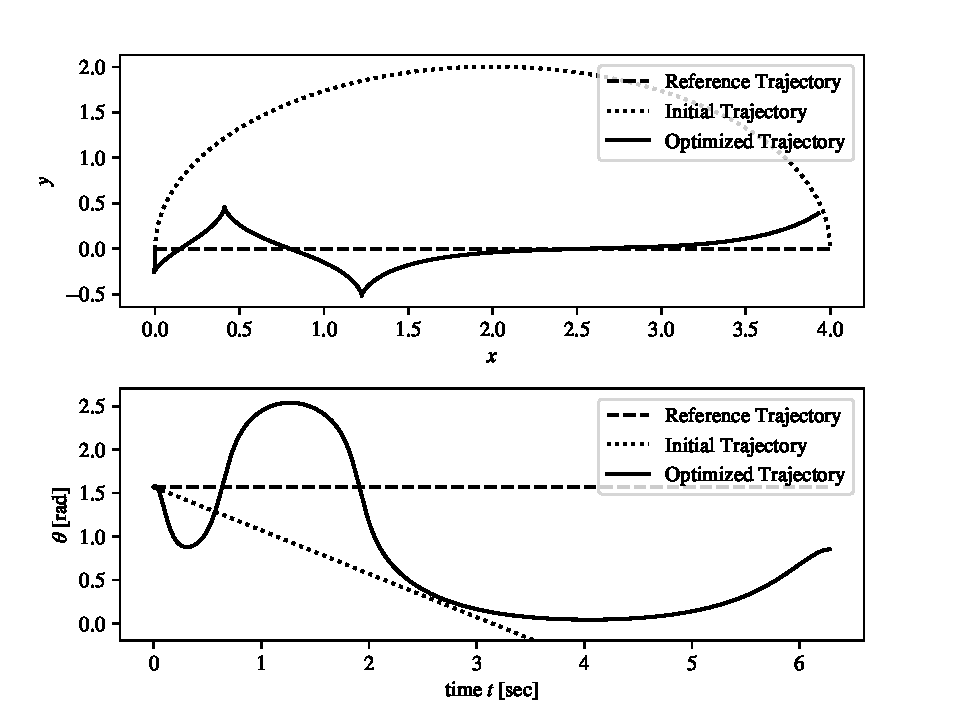
\includegraphics[width=\textwidth]{initial.pdf}
    \caption{Reference trajectory, initial trajectory, and final optimized trajectory}
\end{figure}
\clearpage
Using a quadratic cost function as seen in the lectue:
\begin{equation*}
    J(u(\cdot))=\frac{1}{2} \int_0^T x(t)^{\mathrm{T}} Q x(t)+u(t)^{\mathrm{T}} R u(t) \mathrm{d} t+\frac{1}{2} x(T)^{\mathrm{T}} M x(T)
    \end{equation*}
with weight matrices $Q=\textrm{diag}(100,10,1)$, $R=\textrm{diag}(0.01,0.01)$, $M=\textrm{diag}(1,0,0)$.

\begin{figure}[h]
    \centering
    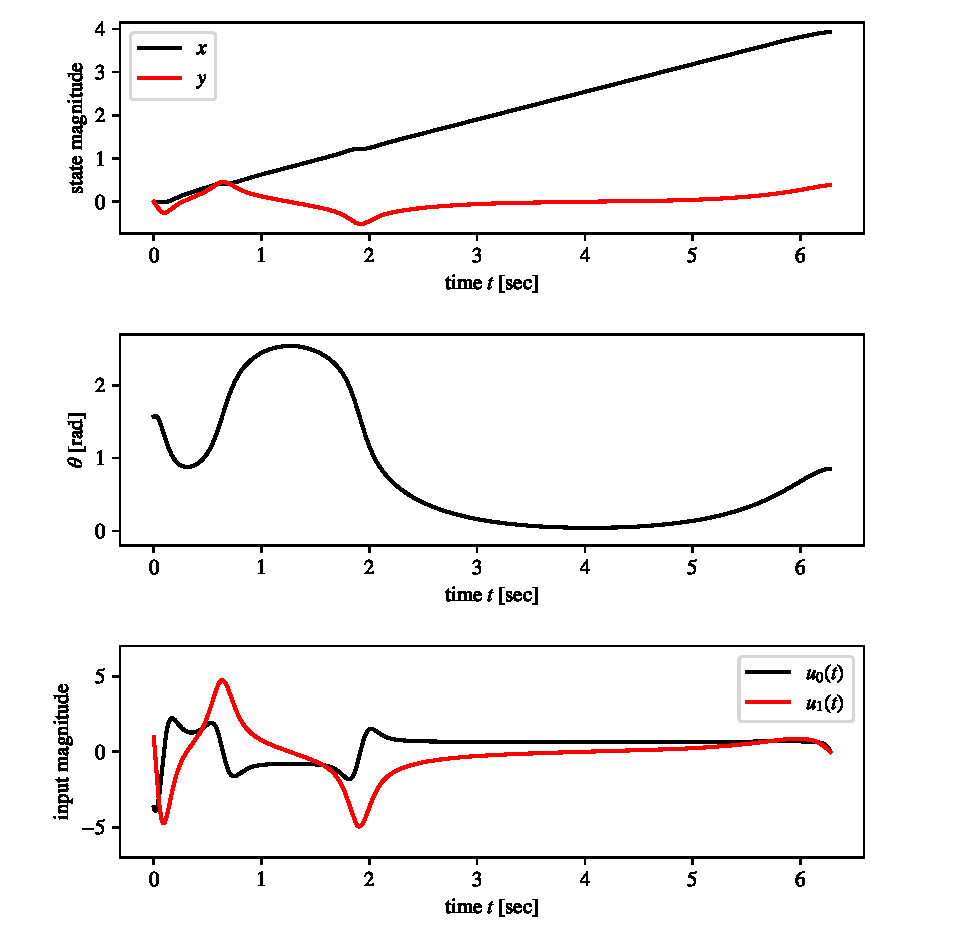
\includegraphics[width=\textwidth]{optimized.pdf}
    \centering
    \caption{Final optimized state and input trajectory}
\end{figure}
\begin{figure}[h]
    \centering
    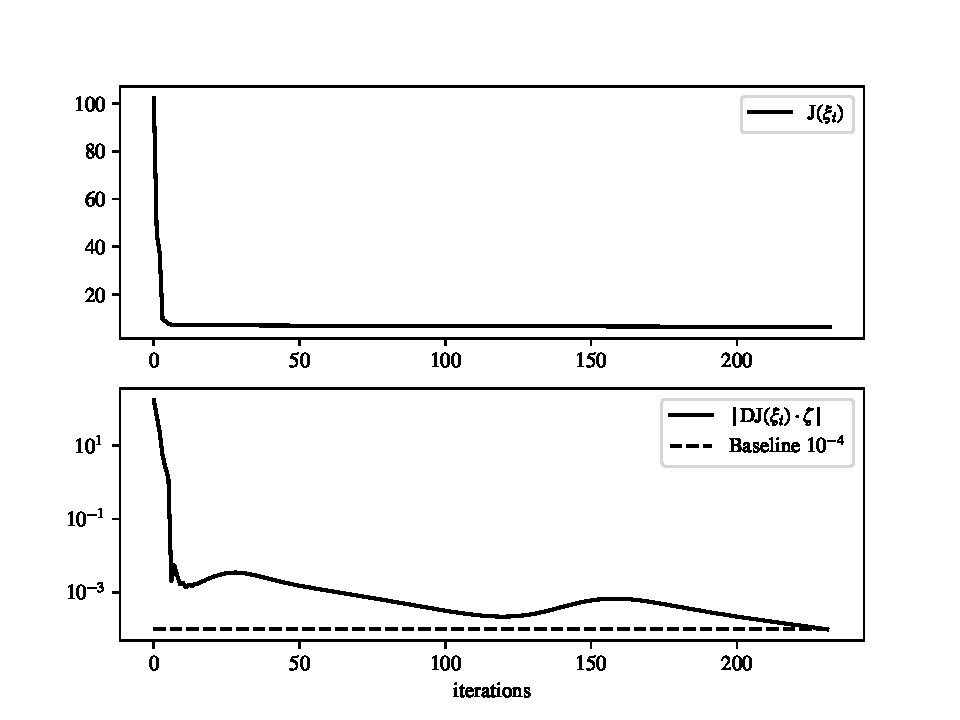
\includegraphics[width=\textwidth]{convergence.pdf}
    \centering
    \caption{Convergence of Cost J$(\xi_i)$ and Cost Derivative DJ$(\xi_i)\cdot\zeta$}
\end{figure}